\documentclass[times, utf8, diplomski]{fer}
\usepackage{booktabs}
\usepackage{graphicx}
\usepackage{algorithm}
\usepackage{algorithmic}
\usepackage{url}
\def\UrlBreaks{\do\/\do-}

\begin{document}

\thesisnumber{2977}

\title{Usporedba algoritama otkrivanja zajednica u društvenim mrežama}

\author{Daniel Marić}

\maketitle

% Ispis stranice s napomenom o umetanju izvornika rada. Uklonite naredbu \izvornik ako želite izbaciti tu stranicu.
\izvornik

% Dodavanje zahvale ili prazne stranice. Ako ne želite dodati zahvalu, naredbu ostavite radi prazne stranice.
\zahvala{Zahvala mentoru prof.dr.sc Goranu Delaču na vodstvu i savjetima tijekom izrade diplomskog rada.}

\tableofcontents

\chapter{Uvod}

Pojavom popularnih internetskih usluga za povezivanje korisnika stvorene su velike mreže društvenih zajednica. Generirane su velike količine podataka iz kojih je moguće izvući mnoštvo korisnih informacija. Takve zajednice sastoje se od puno manjih zajednica koje se po svojim karakteristikama razlikuju od ostalih. Takve zajednice potrebno je pronaći kako bi im se pristupilo na najbolji mogući način. Rješavanje ovog problema važno je i u drugim granama znanosti kao na primjer u sociologiji, biologiji ili računarskoj znanosti gdje su problemi predstavljeni na takav način, pomoću strukture grafa. 

Upravo su grafovi najpogodnija struktura podataka za pristup ovome problemu gdje relevantne značajke, u primjeru društvenih mreža ljude, možemo prikazati pomoću čvorova dok će bridovi predstavljati veze između tih značajki. Više bridova među određenim značajkama značit će da tu mogu postojati obilježja zajednice, npr. u biologiji bi to mogla biti tkiva koja u organima obavljaju sličnu ulogu. 

Rješavanje problema koji su predstavljeni grafovima je vrlo složeno, vremenski i prostorno. Ovakvi grafovi nisu jednostavnog oblika, ali u njima postoje određene pravilnosti koje se mogu iskoristiti. U tu svrhu razvijeno je mnogo algoritama za otkrivanje zajednica koji rezličitim pristupima pokušavaju pronaći rješenje ovog problema. Pojedini algoritmi su bolji od drugih na jednom tipu društvenih mreža ili lošiji na drugom te se zato koriste evaluacijske mjere kojima se procjenjuje koliko je dobro rješenje koje je algoritam pronašao. Što više algoritme testiramo različitim društvenim mrežama i evaluacijskim mjerama dobit ćemo bolji uvid u to kada je bolje koji koristiti. Najpoznatiji algoritam među njima je Newman-Girvanov algoritam koji će se nešto detaljnije opisati uz još nekoliko njih. Sličnim problemima bavili su se radovi Lancichinettija i Fortunata \cite{fortunato2016community} iz 2016. te \cite{lancichinetti2009community} iz 2009. godine.

Unatrag posljednih nekoliko godina uvedeni su zakoni o zaštiti osobnih podataka te je sada znatno teže dobiti pristup korisnim informacijama. Zato se koriste posebni algoritmi za generiranje umjetnih skupova podataka koji će za zadane parametre generirati graf pomoću kojih se mogu provoditi istraživanja. U nastavku rada bit će opisana struktura i svojstva društvenih mreža i zajednica, algoritmi koji pronalaze društvene zajednice, skupovi podataka koji su korišteni u sklopu rada, programsko rješenje koje pokreće i evaluira rješenja algoritama te će se prikazati rezultati do kojih se došlo. 


\begin{figure}
	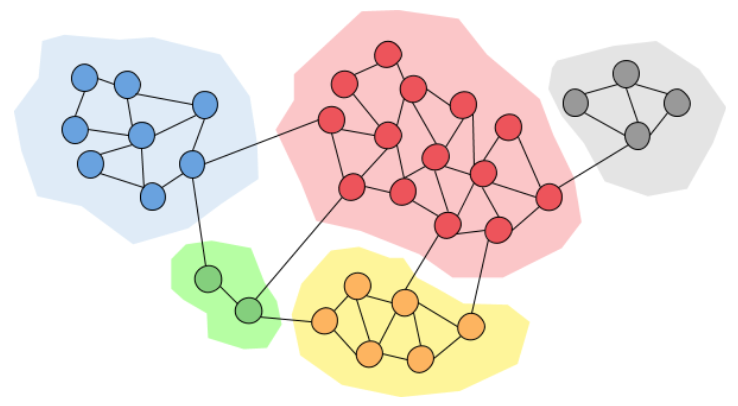
\includegraphics[width=\linewidth]{images/simple-community.png}
	\caption{Primjer grafa nepreklapajućih društvenih zajednica.}
	\label{fig:comm1}
\end{figure}


\chapter{Društvene mreže i zajednice}

Društvene mreže može se pronaći gdje god postoji sustav koji sadrži entitete koji su međusobno povezani. Primjera je mnogo, a neki od njih su: društvene web platforme, email mreže, web stranice koje sadrže poveznice prema drugima, uređaji koji su povezani preko internetske mreže i slično. 
Kako bi se skupina entiteta mogla nazvati društvenom zajednicom među njima mora postojati nekakav tip odnosa. Odnos može biti jednosmjeran ili dvosmjeran te mogu postojati težine kojima se odnosu daje veća ili manja značajnost. Društvene mreže imaju složenu organizacijsku strukturu te se može pretpostaviti svojstvo lokalnosti, koje kaže da ako jedan entitet ima veze prema neka druga dva entiteta onda je vjerojatnost da ta druga dva entiteta imaju vezu, veća od prosječne vjerojatnosti. 

Društvene mreže imaju karakteristično svojstvo grupiranja u strukturu zajednice. Ako se čvorovi mreže mogu podijeliti u nepreklapajuće ili preklapajuće zajednice tako da broj veza između članova zajednice značajno premašuje broj veza između bilo koje dvije zajednice, znači da mreža ima strukturu društvenih zajednica. Mreže koje imaju takvu strukturu često se mogu prikazati i kao hijerarijske strukture. U ovom radu obradit će se mreže koje sadrže nepreklapajuće strukture sa vezama koje nemaju određene težine.

Proces pronalaska društvenih zajednica jedan je od glavnih zadataka u analizama društvenih mreža. Detekcija zajednica može biti vrlo korisna u raznim primjenama kao što je primjerice pronalaženje grupa kojima bi se mogle slati reklame za određene proizvode koji bi ih mogli zanimati umjesto da se svakom pojedincu šalju posebno. Još jedan primjer bio bi preporuka određenih sadržaja koji bi se mogli prikazivati grupama koje pokazuju zanimanja prema sličnim interesima. Primjera ima još mnogo, ali iz ova dva već je vidljivo da se korisne informacije mogu zaključivati iz društvenih mreža. Kako bi društvene mreže pohranili i analizirali u računalu potrebna je prikladna struktura podataka koja će u ovom slučaju biti graf.

\section{Reprezentacija društvenih mreža}

Graf je važna struktura podataka u području računarstva. Pomoću njega moguće je prikazati razne odnose i procese područja bioloških, društvenih i informacijskih sustava. Grafovima se modeliraju vrlo teški problemi kao primjerice problem kineskog poštara ili problem trgovačkog putnika koji je NP težak problem što znači da nema rješenje u polinomnom vremenu.

Prema definiciji jednostavan graf \textit{G} sastoji se od nepraznog konačnog skupa \textit{V(G)}, čije se elemente naziva vrhovi ili čvorovi grafa i konačnog skupa \textit{E(G)} različitih dvočlanih podskupova skupa \textit{V(G)} koji se naziva bridovima \cite{nakic_pavcevic_2019}. Graf može imati najviše $ {n(n-1) \over 2} $ bridova. U radu će se razmatrati jednostavni grafovi koji nemaju petlje i više bridova između istih čvorova. Bridovi će biti bestežinski i neusmjereni. 

Bitna definicija tiče se stupnja vrhova grafa. Stupanj vrha \textit{v} grafa \textit{G} je broj bridova koji su incidentni s \textit{v}. Stupanj vrha označava se sa \textit{deg(v)}. Vrh stupnja 0 zove se izolirani vrh, a vrh stupnja 1 krajnji vrh. \cite{nakic_pavcevic_2019}

Šetnja je graf sa skupom vrhova \textit{V(G) = $ \{x_{1},x_{2},...,x_{l}\} $ } i bridova \textit{E(G) = $ \{x_{0}x_{1},x_{1}x_{2},...,x_{l-1}x_{l}\} $ }. vrhovi $ x_{0} $ i $ x_{l} $ definiraju se kao krajevi dok je \textit{l} duljina šetnje. Ako su svi bridovi šetnje različiti tada se ona naziva staza. Ako su uz to i svi vrhovi različiti onda se takva šetnju naziva putem. Ako put počinje i završava u istom vrhu tada graf sadrži ciklus. Uz pretpostavljena ograničenja najmanji ciklus koji graf u ovom radu može imati je trokut što je često obilježje društvenih mreža.

Definicija puta omogućava definiranje važnog koncepta koji će se pojavljivati u radu pojedinih algoritama. Ako u grafu za svaki par vrhova postoji barem jedan put koji ide od jednog do drugog vrha onda je graf povezan. Ako između vrhova postoji više putova onda je najkraći onaj koji ima najmanju duljinu. Promjer ili dijametar povezanog grafa je najveća udaljenost između bilo koja dva vrha u grafu. Ako ipak postoji barem jedan par vrhova između kojih ne postoji put onda je graf podijeljen u barem dva podgrafa. Svaki maksimalno povezani podgraf zove se komponenta povezanosti. Primjer se može vidjeti na slici \ref{fig:graph}.

\begin{figure}
	\makebox[\textwidth][c]{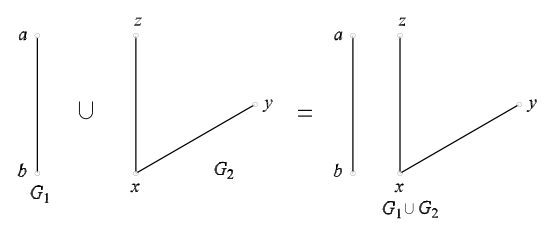
\includegraphics[width=0.7\textwidth]{images/nepovezani-graf.png}}
	%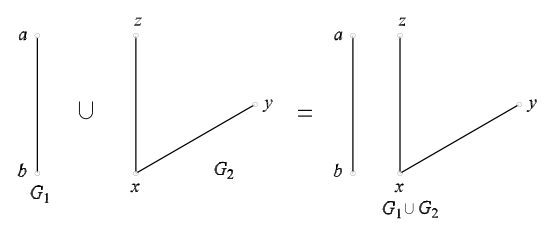
\includegraphics[width=0.7\textwidth]{images/nepovezani-graf.png}
	\caption{Primjer nepovezanog grafa}
	\label{fig:graph}
\end{figure}

Grafovi se mogu pohranjivati u obliku matrice susjedstva gdje su dva vrha, \textit{i} i \textit{j} susjedna ako im je element matrice \textit{A{ij}} jednak 1, a inače 0. Zbog pretpostavke da ne postoje petlje na dijagonali matrice susjedstva svi su elementi nule. Za reprezentaciju neusmjerenog grafa matrica susjedstva je simetrična što znači da je dovoljno pohraniti samo jedan trokut matrice, iznad ili ispod dijagonale. Suma elemenata \textit{i}-tog retka ili stupca jednaka je stupnju vrha \textit{i}

Jednostavniji oblik pohrane liste susjedstva koja se koristi tako da se pohranjuje skup susjednih bridova koji predstavljaju graf. Lista susjedstva je prostorno učinkovitija od matrice susjedstva kada su u pitanju rijetki grafovi kod kojih većina vrhova nije međusobno povezana. Prostorno zauzeće ovisi o broju vrhova i bridova u grafu, dok je kod matrice susjedstva uvijek proporcionalno kvadratu broja vrhova.


\section{Obilježja društvenih zajednica} 

Društvene zajednice moguće je definirati na nekoliko načina sa različitih stajališta, ali ne postoji niti jedna univerzalno prihvaćena definicija. Definiranje vrlo često ovisi o problemu koji se promatra zajedno sa specifičnim detaljima i primjenama gdje se pojam zajednice koristi. Prema radu \cite{fortunato2010community} zajednice je moguće promatrati iz lokalne i globalne perspektive.

Iz lokalne perspektive zajednica se može promatrati kao grupa entiteta koji su međusobno sličniji u odnosu na ostale entitete skupa podataka. Zajednica se formira tako što slični elementi imaju mnogo više interakcija sa članovima unutar zajednice u odnosu na one izvan. Zajednica se može smatrati kao autonomna skupina te ima smisla u određenim situacijama evaluirati svaku zasebno od ostatka društvene mreže. Stroga definicija društvene mreže kaže kako je društvena zajednica podgraf u kojem su svi članovi međusobno u interakciji \cite{luce1949method}. Takva definicija odgovara terminu klike u teoriji grafova koji označava skup vrhova koji su svi međusobno susjedni. Najjednostavniji primjer klike je trokut i oni se pojavljuju u svim društvenim mrežama. Veće klike od trokuta se pojavljuju rjeđe te ovakva definicija tako postaje manje praktična u stvarnim primjerima. Još jedan problem klike je to što su tada svi vrhovi simetrični bez mogućnosti razlikovanja njihovih svojstava. U praktičnim primjerima očekuje se da među vrhovima postoji određena hijerarhijska struktura sa više i manje važnim čvorovima. Moguće je relaksirati pojam klike. Mogućnost je iskoristiti doseg i duljinu puta između čvorova. n-klika je takav podgraf da niti jedan par vrhova nije međusobno udaljen za više od \textit{n} koraka i skup je maksimalan u smislu da niti jedan drugi čvor nije udaljen za više od \textit{n} od svakog čvora iz podgrafa. Može se primijetiti da članovi podgrafa mogu biti povezani preko posrednika koji nije član grupe te onda n-klika ipak nije dovoljno dobra definicija. Definicija n-klana to popravlja. n-klan je n-klika u kojoj je dijametar podgrafa manji ili jednak \textit{n}. Takva definicija ima problem što u njoj i dalje postoji zahtjev n-klike te se tako dolazi do definicije n-kluba. n-klub je podgraf gdje je dijametar manji ili jednak \textit{n}. Tada je i svaki n-klan i n-klub i n-klika.

Iz globalne perspektive zajednica se može definirati promatrajući graf u cjelini. Takve definicije koriste se u slučajevima kada su zajednice dijelovi sustava bez kojih bi njegovo funkcioniranje bilo značajno izmijenjeno. Definicije se najčešće izvode indirektno, iz algoritama prema kojem je neko svojstvo iskorišteno kako bi se zajednice otkrile. Moguće je definirati null model koji će odgovarati prema određenim strukturnim karakteristikama, ali inače je slučajni graf. Model se tada koristi za usporedbu kako bi se odredilo ima li promatrani graf strukture zajednica. Poznati null model grafa predložili su Newman i Girvan koji se dobije tako da se u početnom grafu slučajno prespajaju bridovi pod uvjetom da stupanj svakog vrha ostane isti kao u početnom grafu. Iz njega je proizašla definicija modularnosti, odnosno funkcije kojom je moguće ocijeniti kvalitetu pronađenih zajednica u grafu. Modularnost je važna mjera jer ima nekoliko primjena u području otkrivanja zajednica. Koristi se kao mjera koja određuje koliko su kvalitetne pronađene grupe u mreži, ali i kao sastavni dio poznatog Girvan-Newmanovog algoritma \cite{fortunato2010community}.

\section{Small-world mreže}

Small-world mreže imaju obilježja dva tipa mreža. Prva mreža je slučajna mreža za koju je karakteristično što je prosječna udaljenost između dva vrha vrlo mala. Druga mreža je rešetkasta u obliku prstena gdje je svaki čvor susjedan sa $\dfrac{n}{2}$ čvorova sa svake strane. Small-world mreža posjeduje svojstva tih grafova te se pomoću njih može procijeniti u kojoj je mjeri mreža zaista small-world. Na temelju tih svojstava nastao je i Watts–Strogatz model koji služi za generiranje slučajnih grafova društvenih mreža što se može iskoristiti u testiranjima raznih algoritama za detekciju zajednica. Primjeri mreža prikazani su na slici \ref{fig:small-world}.

\begin{figure}
	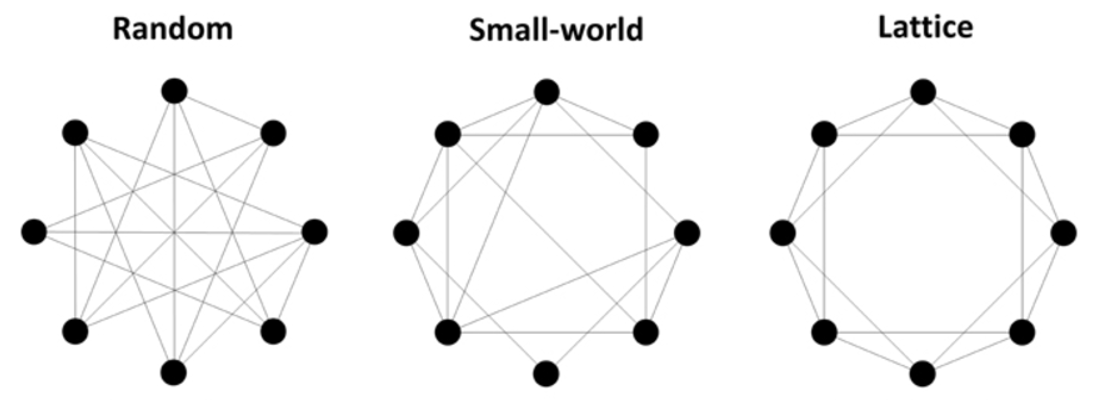
\includegraphics[width=\linewidth]{images/small-world.png}
	\caption{Primjeri slučajnog, small-world i rešetkastog grafa.}
	\label{fig:small-world}
\end{figure}

Small-world mreža je graf u kojem većina čvorova nisu susjedi, ali susjedi nekog čvora imaju veliku vjerojatnost da su i oni susjedi te se do svakog čvora može doći kroz nekoliko koraka što znači da bilo koja dva čvora imaju kratku međusobnu udaljenost. Specifično je što se ona za dva slučajno izabrana čvora te za fiksiran prosječan stupanj vrha povećava proporcionalno logaritmu broja čvorova u grafu dok koeficijent grupiranja nije malen. Small-world mreže sadrže klike i grupe koje su gotovo klike što proizlazi iz visokog koeficijenta grupiranja. Društvene mreže posjeduju svojstva small-world mreže.

Koeficijent grupiranja je mjera stupnja u kojem čvorovi u grafu teže grupiranju. Postoje dvije verzije mjere, lokalna i globalna. U lokalnoj verziji mjera se računa za pojedini čvor te govori u kolikoj je on mjeri grupiran sa svojim susjedima. Mjera se za čvor \textit{i} računa kao suma broja veza koje postoje između susjeda promatranog čvora podijeljeno sa brojem svih mogućih veza,
\begin{equation}
C_{i} = \dfrac{2 \mid e_{jk}:v_{j},v_{k} \in N_{i}, e_{jk} \in E \mid}{k_{i}(k_{i}-1)}.
\end{equation}
 Ako iz formule maknemo koeficijent 2 tada se ona može koristiti za usmjerene grafove.
Globalni koeficijent grupiranja daje informaciju o grupiranju u cijeloj društvenoj mreži. Temelji se na trojkama čvorova. Trojku čine promatrani čvor i druga dva čvora. Ako su povezani sa dva brida zovu se otvorena trojka, a ako su povezani sa tri zovu se zatvorena trojka što znači da jedan trokut čine tri trojke. Koeficijent se tada računa kao broj zatvorenih trojki podijeljen sa ukupnim brojem trojki, 
\begin{equation}
 C = \dfrac{broj \; zatvorenih \; trojki}{ukupan \; broj \; trojki}.
\end{equation}
Formula je primjenjiva i na usmjerene i neusmjerene grafove.

Kratka prosječna duljina puta između čvorova znači da postoje čvorovi sa velikim brojem veza odnosno visokim stupnjem. Takvi čvorovi nazivaju se sabirnice te služe kao posrednici u mnogim putevima između ostalih čvorova. Primjer iz stvarnog svijeta može se pronaći u zračnim letovima između gradova. Na putovanju između dva grada vrlo često nije potrebno više od tri leta jer mnogo letova ide preko jednog velikog grada sa puno letova prema drugima. 

Koliko mreža pripada small-world mreži može se izraziti pomoću small-koeficijenta, \textit{$\sigma$}, koji se računa tako da se uspoređuju koeficijent grupiranja i karakteristična duljina puta u mreži sa slučajnim grafom koji ima jednak prosječan stupanj vrhova. Za karakterističnu duljinu puta najčešće se koristi prosječna minimalna udaljenost između vrhova. Koeficijent se računa prema formuli:
\begin{equation}
 \sigma = \dfrac{\dfrac{C}{C_{r}}}{\dfrac{L}{L_{r}}}.
\end{equation}

$ C $ i $ L $ su mjera grupiranja i prosječna duljina puta u promatranoj mreži dok su  $ C_{r} $ i $ L_{r} $ su mjera grupiranja i prosječna duljina puta u slučajnom grafu. Ako je $ \sigma $ > 1 tada se može smatrati da je mreža small-world. No mjera pokazuje lošu otpornost na rast broja čvorova u mreži \cite{telesford2011ubiquity}.

Druga mjera kojom se može izmjeriti koliko je mreža small-world uspoređuje promatranu mrežu s mrežom rešetkastog oblika (eng. lattice network) i slučajnom mrežom. Mjera kombinira karakterističnu duljinu puta i koeficijent grupiranja sa koeficijentom grupiranja rešetkaste mreže i karakterističnom duljinom puta ekvivalentnog slučajnog grafa prema sljedećoj formuli:
\begin{equation}
	\omega = \dfrac{L_{r}}{L} - \dfrac{C}{C_{l}}
\end{equation}
Ovakva definicija nije osjetljiva na mjeru $ C_{r} $ koja nije primjerena za mjerenje je li mreža small-world jer slučajni graf nema svojstva grupiranja. Vrijednosti koeficijenta $\omega$ ograničene su na interval između -1 i 1 bez obzira na veličinu mreže. Za vrijednost oko 0 može se smatrati da je mreža small-world što znači da je $ L \approx L_{r} $ i $ C \approx C_{l} $. Pozitivne vrijednosti ukazuju na to da graf ima više sličnosti sa slučajnim grafom, dok negativne na to da je graf pravilnijeg, rešetkastog oblika \cite{telesford2011ubiquity}.


Posljednja mjera koja kvantificira small-world mjeru normalizira koeficijent grupiranja i duljinu puta mreže relativno u odnosu na karakteristike ekvivalentne rešetkaste i slučajne mreže. Small World Index (SWI) računa se na sljedeći način:
\begin{equation}
	SWI = \dfrac{L - L_{l}}{L_{r} - L_{l}} \cdot \dfrac{C - C_{r}}{C_{l} - C{r}}
\end{equation} 
Mjera ima interval rezultata između 0 i 1. Što je bliže 1 to je više vjerojatno da je mreža small-world. Vrlo je vjerojatno da ne postoji mreža koja bi imala SWI = 1, ali ideja mjere je izmjeriti small-world svojstvo na način koji bi teoretski činio mrežu idealnom small-world mrežom gdje vrijedi da je $ C \approx C_{l} $ i $ L \approx L_{r} $.





\chapter{Algoritmi otkrivanja društvenih zajednica}

Ključan dio u pronalasku društvenih zajednica u društvenim mrežama su algoritmi koji ih otkrivaju. Oni moraju biti pouzdani i učinkoviti, ali se i izvršavati u prihvatljivom vremenskom okviru. Algoritmi se testiraju na brojnim skupovima podataka uz prikladne evaluacijske mjere kako bi se zaključilo u kojim uvjetima koji algoritam daje najbolje rješenje. 

Grafove koji predstavljaju društvene zajednice teško je prikazati u ravnini ako teže stvarnim veličinama koje se kreću u tisućama čvorova, a često i mnogo više, što znači da se ne može iz ljuske perspektive odrediti kako bi dobar raspored zajednica izgledao. To znači da su algoritmi koji pronalaze društvene zajednice nenadzirani algoritmi koji sami, bez primjera za učenje i unaprijednog znanja o njima pokušavaju pronaći rješenje. U društvenim mrežama algoritmi koriste topološke karakteristike i specifičnosti koje posjeduju ovakvi tipovi mreža. 

Dvije važne tehnike na kojima se temelji većina algoritama su particioniranje i grupiranje. Particioniranje grafova je proces u kojem se graf dijeli na unaprijed određeni broj manjih komponenti pomoću određenog svojstva. Svojstvo koje se može iskoristiti je minimalni rez. Ono se koristi tako da se graf podijeli na dva ili više razdvojenih podgrafova, a veličina reza koja se pokušava minimizirati je broj bridova koje je potrebno ukloniti da bi to ostvarili. Potrebno je odrediti i svojstvo koje bi odredilo veličinu komponenti kao primjerice minimalan ukupan stupanj vrhova kako bi se dobila rješenja koja imaju smisla. Zbog takvih zahtjeva ovakav pristup najčešće nije prihvatljiv jer broj zajednica nije moguće unaprijed odrediti.
Grupiranje je proces u kojem se entitete koji imaju zajedničke karakteristike svrstava u iste grupe. Pronalaženje grupa može dati informacije o skrivenim značajkama, vezama i svojstvima članova te koliko su međusobno čvrsto povezani. U hijerarhijskom grupiranju stvara se hijerarhija među zajednicama. Proces se može odvijati na dva načina, aglomerativni ili divizivni. U aglomerativnom načinu se koristi pristup koji ide od dna prema vrhu te se određeni čvor dodaje drugim sličnim čvorovima te se koristi određeni kriterij sličnosti. U divizivnom načinu veće grupe dijele se na manje uz korištenje određene mjere koja govori koliko je dobra trenutačna podjela prema kojoj će se odrediti konačan rezultat.



\section{Girvan-Newmanov algoritam}

Veliko zanimanje i rast aktivnosti znanstvene zajednice u području društvenih mreža potaknuo je rad Girvana i Newmana iz 2002. godine \cite{girvan2002community} u kojem su predstavili novi algoritam koji se po njima i naziva. Dotad poznati algoritmi pokušavali su pronalaženje zajednica riješiti tako da bi provodili hijerarhijsko grupiranje. U početnom koraku kreće se od nepovezanog grafa te se za svaki par vrhova računa težina koja predstavlja koliko su vrhovi bliski. Tada se bridovi se dodaju jedan po jedan počevši od onih vrhova čija je bliskost najveća. Postoji više načina kako izračunati bliskost i temelje se na broju puteva između čvorova, npr. broj vršno nezavisnih putova ili bridno nezavisnih putova i slično. Takve definicije ipak u nekim slučajevima nisu uspješne i daju krive rezultate. Događa se da se vrhovi koji su na rubovima zajednice, povezani jednim bridom prema ostatku mreže izdvajaju iz zajednice kojoj pripadaju i ostaju potpuno izolirani od svih zajednica. Girvan-Newmanov algoritam pokušava suprotno, pronaći bridove koji što manje doprinose povezanosti unutar zajednica. 

Algoritam traži bridove koji povezuju zajednice te ih kroz iteracije uklanja i izolira zajednice. Za pronalazak bridova koristi se mjera različitosti, u ovom slučaju mjera bridne centralnosti. Njezina vrijednost računa se za svaki brid tako što se za sve parove vrhova odredi najkraći put te se svim bridovima koji se nalaze u tom putu dodaje vrijednost 1. Ako postoji $N$ najkraćih putova između vrhova onda se u svim putevima svakom bridu vrijednost povećava za $ \dfrac{1}{N} $. Bridna centralnost svakog vrha na početku je postavljena na 0. Postupak se ponavlja dok god postoji bridova u grafu. Izračunavanje bridne centralnosti je skupa operacija jer je potrebno za svaki par vrhova u svakoj iteraciji pronaći najkraći put te odrediti bridne centralnosti Mora se provoditi u svakom koraku jer se inače mogu dogoditi pogreške u koracima algoritma zato što se mreža prilagođava novom stanju nakon uklanjanja svakog brida. Takva situacija može se dogoditi ako su dvije zajednice povezane sa više bridova. Tada je prema algoritmu, sigurno da će barem jedan od tih bridova imati visoku bridnu centralnost te se zato nakon njegovog uklanjanja vrijednost mjere mora ponovno odrediti, a onda će jedan od preostalih bridova imati najvišu vrijednost. Moguće je uštedjeti nešto resursa tako što se bridna centralnost izračunava samo za one vrhova na koje je uklanjanje prethodnog brida imalo utjecaja. 

\bigskip
\begin{algorithm}
\caption{Girvan-Newmanov algoritam}
\begin{algorithmic}[1]
	\STATE izračunati mjeru različitosti za sve bridove u grafu
	\STATE ukloniti brid sa najvećom vrijednosti mjere različitosti
	\STATE za svaki brid izračunati mjeru različitosti nakon uklanjanja brida
	\STATE ponavljati korake 2 i 3 dok ima bridova u grafu
\end{algorithmic}
\end{algorithm}
\bigskip

Konačno rješenje algoritma određuje se tako što se u svakoj iteraciji računa modularnost za trenutnu podjelu grafa. Modularnost je mjera koja se koristi za procjenu jakosti veza unutar zajednice i jakosti veza među zajednicama. Njome je moguće izmjeriti koliko je određena podjela grafa kvalitetna. Ona podjela koja ima najvišu vrijednost na kraju algoritma uzima se kao rezultat. O modularnosti i ostalim mjerama mjerenju rezultata više će biti rečeno u poglavlju \ref{vrednovanja_i_rezultati} koje se bavi vrednovanjem rezultata algoritama.


Postupak traženja zajednica tijekom rada algoritma može se predstaviti dendogramom. Dendogram je prema strukturi stablo gdje su listovi pojedini vrhovi mreže. Prema vrhu stabla vrhovi se spajaju u zajednice te konačno u cijelu strukturu grafa. Vrhovi povezani na nižim razinama imaju snažnije međusobne veze. Rez kroz stablo na bilo kojoj razini daje skup zajednica koji u tom trenutku postoji. Gdje stablo odrezati određuju se pomoću modularnosti. Primjer je prikazan na slici \ref{fig:dendogram}.

\begin{figure}
	%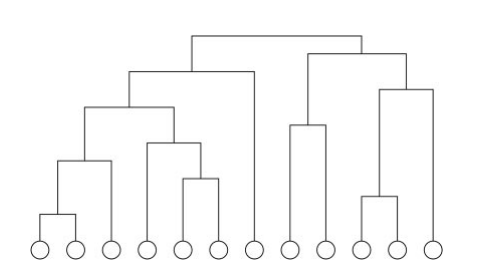
\includegraphics[width=\linewidth]{images/dendogram.png}
	\makebox[\textwidth][c]{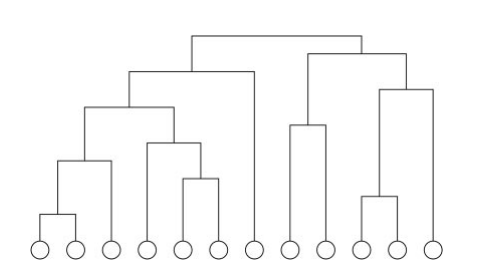
\includegraphics[width=0.8\textwidth]{images/dendogram.png}}
	\caption{Primjer hijerarhijskog stabla. Moguće je po koracima vidjeti kada je koji brid uklonjen iz mreže te kako su grupe nastale.}
	\label{fig:dendogram}
\end{figure}

Za graf od \textit{m} bridova i \textit{n} vrhova složenost algoritma u najgorem slučaju je $\mathcal{O}(m^{2}n)$. Potrebno je u svakom koraku algoritma ponovno izračunati mjeru različitosti što ima velik utjecaj na povećanje složenosti. U boljim slučajevima, kada se mreža nakon nekoliko iteracija razdvoji u nekoliko komponenti izvođenje algoritma znatno se ubrzava. U nekoliko slučajeva isprobana je strategija da se mjera različitosti izračuna jednom, na početku izvođenja algoritma, ali u radu \cite{girvan2002community} se pokazalo da takav postupak ne daje ispravna rješenja.

\pagebreak

\section{Louvain algoritam}

Algoritam osmišljen na sveučilištu u Louvainu stvoren je kako bi nadmašio dotad poznate algoritme u području otkrivanja zajednica. Objavljen je u radu \cite{blondel2008fast}, 2008. godine. Algoritam je testiran pronalaženjem zajednica u belgijskoj telefonskoj mreži od 2.6 milijuna korisnika te analiziranjem web grafa od 118 milijuna čvorova i više od milijardu bridova za koji je rješenje izračunao u 152 minute. Kapaciteti algoritma i testiranih mreža bili su ograničeni samo dostupnim kapacitetom računalnih resursa, a ne vremenom potrebnim za računanje. Algoritam se koristi heurističkom metodom koja se temelji na optimizacije modularnosti. 

Rad algoritma podijeljen je u dvije faze koje se ponavljaju kroz iteracije. U prvom koraku, za graf od \textit{N} čvorova, svaki čvor pripada zajednici u kojoj je samo on član što znači da u početku postoji onoliko zajednica koliko graf ima čvorova. Tada se za svaki čvor \textit{i} promatraju njegovi susjedi \textit{j} te se računa promjena modularnosti koja bi se dogodila ako se čvor \textit{i} premjesti u zajednicu čvora \textit{j}. Čvor \textit{i} se premješta u zajednicu za koju je promjena maksimalna i pozitivna, odnosno modularnost raste. Ako je nema rasta promatrani čvor ostaje u dodijeljenoj zajednici. Proces se ponavlja slijedno dok god postoje poboljšanja. Moguće je da se svi čvorovi razmatraju kroz nekoliko iteracija. Kada se u iteraciji ne dogodi niti jedno poboljšanje algoritam završava prvu fazu. U radu \cite{blondel2008fast} pokazalo se kako redoslijed čvorova nema značajnijeg utjecaja na rezultat, ali se može uštedjeti na vremenu izračunavanja. Dio učinkovitosti algoritma proizlazi iz jednostavnog računanja promjene modularnosti tijekom premještanja čvora \textit{i} u grupu \textit{C} koja se dobiva prema sljedećem izrazu: 
\begin{equation}
	\Delta Q =  \bigg[ \frac{\sum_{in} + k_{i,in}}{2m} - \bigg( \dfrac{\sum_{tot} + k_{i} }{2m} \bigg)^{2} \bigg] 
	- 
	\bigg[ \dfrac{\sum_{in}}{2m} - \big( \dfrac{\sum_{tot}}{2m} \big)^{2} - \bigg( \dfrac{k_{i}}{2m} \bigg)^{2} \bigg] .
\end{equation}
\bigskip
$\sum_{in}$ predstavlja sumu težina bridova, \textit{C}, $\sum_{tot}$ je suma težina bridova koji su povezani sa čvorovima u zajednici \textit{C}, $k_{i}$ je suma težina bridova koji su incidentni sa čvorom \textit{i}. $k_{i,in}$ je suma težina bridova koji povezuju čvor \textit{i} sa zajednicom \textit{C} i \textit{m} je broj bridova u cijeloj mreži. U primjeni se promjena modularnosti računa tako što se čvor \textit{i} premješta iz trenutne zajednice u susjedne te se promatra kako se vrijednosti ponašaju.

\bigskip
\begin{algorithm}
	\caption{Louvain algoritam}
	\begin{algorithmic}[1]
		\REQUIRE graf \textit{G}
		\REPEAT 
		\STATE svaki čvor grafa $G$ dodijeliti u vlastitu zajednicu
		\WHILE{postoje čvorovi koji se premještaju}
		\FORALL{čvor $n$ grafa $G$}
		\STATE postaviti čvor u susjednu zajednicu uključujući i trenutnu tako da se rast modularnosti maksimizira
		\ENDFOR
		\ENDWHILE
		\IF{nova modularnost veća od prethodne} 
		\STATE {graf $G$ postaje novi graf sa čvorovima koje čine prethodno dobivene zajednice} 
		\ELSE \STATE{kraj} 
		\ENDIF
		\UNTIL{}
	\end{algorithmic}
\end{algorithm}
\bigskip

Druga faza algoritma sastoji se od građenja nove mreže čiji čvorovi postaju zajednice koje su pronađene tijekom prve faze. Kako bi se dobio cjelovit graf potrebno je nove čvorove povezati bridovima. Brid se dodaje tako da spaja zajednice čiji su čvorovi bili susjedni te mu je težina suma težina tih bridova. Ako je brid bio unutar zajednice predstavlja se petljom koju je moguće izostaviti. U početnom koraku za graf koji nema određene težine bridova, težine se mogu postaviti na 1. Kada druga faza završi ponavlja se prva faza na novonastalu mrežu. Ako se promotri rad algoritma te činjenicu da je u početku svaki čvor jedna zajednica, onda se može zaključiti da se broj zajednica kroz iteracije smanjuje te je resursno najzahtjevnija prva iteracija. Faze se ponavljaju dokle god ima promjena u strukturi zajednica te modularnost ne postigne maksimum. Može se primijetiti da se kroz proces algoritma prirodno uključio pojam hijerarhije kada se manje zajednice spajaju u veće. Visina hijerarhije ovisi o broju iteracija algoritma te je uobičajeno manji broj.

Algoritam je jednostavan, intuitivan i jednostavan za implementaciju te radi nenadzirano. Složenosti je $\mathcal{O}(n \cdot log{}n)$. Zbog pohlepne optimizacije, jednostavnog izračuna promjene modularnosti i naglog rasta broj zajednica brzo se izvršava što se dodatno ističe u mrežama su rijetke i koje imaju čvrste strukture zajednica. Postoji problem koji se događa zbog modularnosti koja ima problem u prepoznavanju manjih zajednica što se naziva rezolucijski limit. Njegov utjecaj ublažen je time što algoritam u početnom koraku kreće od situacije gdje je svaki čvor u svojoj zajednici te je vjerojatnost da će dvije različite zajednice biti spojene tako da se čvorovi premještaju jedan po jedan vrlo niska. Ako zajednice pokažu veliku bliskost mogu se spojiti kasnije nakon što se čvorovi u njima združe. Takvo ponašanje ističe se u slučaju klika koje konačno budu u jednoj zajednici, ali su razdvojene u početnim prolazima što znači da je moguće dobiti uvid u rješenja međukoraka algoritma te se krajnjem korisniku tako može pružiti uvid u promatranje zajednica na određenoj rezoluciji, odnosno hijerarhijskoj razini.


\section{Surprise algoritam}

Surprise algoritam uvodi novu mjeru kvalitete podjele zajednica u mreži. U radovima \cite{blondel2008fast} i \cite{gamermann2022algorithm} prikazano je kako modularnost ima određenih nedostataka. Događa se problem s rezolucijom te se manje zajednice združuju s većima pri čemu može doći do situacije da povezanost čvorova unutar zajednice postaje slaba. Modularnost također posjeduje mnogo sličnih lokalnih maksimuma što znatno otežava pronalaženje globalnog. Moguća je i situacija u kojoj se za strukturno vrlo različite podjele zajednica dobivaju slične vrijednosti modularnosti. Mjera koja bi trebala riješiti navedene probleme naziva se surprise. Predstavljena je u radu \cite{aldecoa2010jerarca} kao mjera za procjenu kvalitete pronađenih zajednica algoritama hijerarijskog grupiranja. U mnogim radovima mjera je korištena za ocjenjivanje rezultata raznih algoritama, ali u radu \cite{gamermann2022algorithm} je iskorištena kao dio algoritma.


U grafu sa \textit{K} čvorova i \textit{n} bridova podijeljenih u $N_{c}$ zajednica takvih da je $l$ bridova mreže povezuje vrhove iste zajednice surprise mjera definira se na sljedeći način:

\begin{equation}
	S = - ln \sum_{j = l}^{min(M,m)} \frac{ {M \choose j} {F-m \choose n-j} }{ {F \choose n}}.
\end{equation}
Mjera je hipergeometrijska distribucija gdje $F$ predstavlja maksimalan broj mogućih bridova u mreži, $F = \frac{K(K-1)}{2}$ dok je $M$ maksimalan moguć broj bridova unutar $N_{c}$ zajednica gdje je broj čvorova unutar zajednice $i$, $c_{i}$. $M$ se računa prema sljedećem izrazu:
\begin{equation}
	M = \sum_{i=1}^{N_{c}} \frac{c_{i}(c_{i}-1)}{2}.
\end{equation} 
Surprise mjeru može se zamisliti kao mjerenje koliko je malo vjerojatno, iznenađujuće, pronaći zajednicu sa $l$ bridova unutar nje kao u promatranoj mreži. Postupak se može promatrati kao posuda sa $F$ loptica gdje svaka loptica predstavlja jedan od mogućih bridova unutar mreže, gdje ih je $M$ crveno koji predstavljaju moguće bridove unutar zajednice, a $F-M$ ih je plavih koji predstavljaju bridove između različitih zajednica. Iz posude se izvlači $n$ loptica koje predstavljaju stvaran broj bridova u grafu. Suma s desne strane jednadžbe je vjerojatnost izvlačenja barem $l$ crvenih loptica. Obično vrijedi da je $M << F$ te vjerojatnost izvlačenja crvene loptice može biti niska.

Surprise algoritam detekcije zajednica sličan je Louvain algoritmu. U početnom koraku mreža se podijeli u onoliko zajednica koliko ima čvorova. Tada algoritam pokušava premještanjem čvorova pronaći takvu raspodjelu koja će maksimizirati vrijednost surprise mjere. Razlika u odnosu na Louvain algoritam je što se premještanje čvorova može obavljati na tri načina. Dvije zajednice mogu biti spojene u jednu, jedan čvor se može premjestiti iz jedne u drugu zajednicu ili se čvor može izdvojiti u novu grupu. Druge dvije operacije mogu se pokrenuti rekurzivno za svaku zajednicu što algoritmu daje dodatnu snagu. Time je moguće otkriti manje podgrupe unutar zajednice te ih potencijalno izdvojiti u novu zajednicu ili pridružiti nekoj od postojećih. Operacije također pomažu algoritmu u izbjegavanju lokalnih maksimuma.

Algoritam je pohlepan što znači da prati svako poboljšanje vrijednosti surprise mjere koje pronađe sve dok ih više ne može naći. Istraživanja u radu \cite{gamermann2022algorithm} su pokazala da neke druge strategije u biranju smjera u kojem će surprise mjere rasti nisu pokazala bolje rezultate od pohlepne strategije dok su bile računalno zahtjevnije, no mogu se koristiti u završnim koracima algoritma kada razlike u rastu mjere postaju male.


\begin{algorithm}
	\caption{Surprise algoritam}
	\begin{algorithmic}[1]
		\REQUIRE mreža \textit{G}
		\WHILE{postoje promjene u mreži} 
			\FOR{svaka zajednica u mreži} 
				\FOR{svaki čvor u zajednici} 
					\FOR{svaki susjed čvora} 
						\IF{zajednica susjeda različita od trenutne zajednice} 
							\STATE {pokušati spojiti zajednice ili izmijenti čvorove između njih} 
						\ENDIF
					\ENDFOR
				\ENDFOR 
				\WHILE{postoje promjene} 
					\STATE{izdvojiti čvor iz zajednice} 
				\ENDWHILE
				\WHILE{postoje promjene} 
					\STATE{izdvojiti podzajednicu iz zajednice} 
				\ENDWHILE
				\WHILE{postoje promjene} 
					 \FOR{svaku drugu zajednicu u mreži} 
					 	\STATE {pokušati premjestiti podzajednicu u drugu zajednicu} 
					 \ENDFOR
				\ENDWHILE				
			\ENDFOR
		\ENDWHILE
	\end{algorithmic}
\end{algorithm}

Algoritam iterira kroz zajednice dok god se događaju promjene u strukturi zajednica. U svakoj zajednici prolazi kroz sve čvorove te ih pokušava pridružiti susjednima pojedinačno ili kao čitavu zajednicu. Potom pokušava iz svake zajednice izdvojiti čvor, izdvojiti podzajednicu ili je premjestiti u drugu zajednicu. Postojanje promjene znači da je određena operacija podigla vrijednost surprise mjere za novu raspodjelu.

Postoji velik broj kombinacija kako se čvorovi mogu podijeliti u zajednice te ih nije moguće sve provjeriti. Važno je promotriti kako se konfiguracija zajednica ponaša u situacijama kada su lokalni maksimumi slične vrijednosti te koliko su blizu globalnog. U radu \cite{gamermann2022algorithm} je pokazano da surprise algoritam ne pati od problema degeneracije ako je lokalni maksimum blizu globalnog što znači da i u slučajevima kada maksimum surprise mjere nije postignut konfiguracija mreže je reprezentativna što za modularnost nije vrijedilo. Ipak ne postoji garancija da će globalni maksimum biti pronađen, ali algoritam uz surprise mjeru trebao bi dati bolje rješenje u odnosu na onaj s modularnosti.



\section{Leiden algoritam}

Leiden algoritam osmišljen kako bi ispravio nedostatke Louvain algoritma. Lovain algoritam može kao konačan rezultat pronaći slabo povezane zajednice u situacijama gdje su one i iznad i ispod ranije spomenutog problema s rezolucijskom granicom. Algoritam može premjestiti čvor koji je predstavljao most između komponenti trenutne zajednice u drugu zajednicu dok ostali čvorovi ostaju u zajednici i ne premještaju se u neku od prikladnijih u tom trenutku. Događanje navedenog primjera izbjegava se u slučajevima kada je zajednica iznutra čvrsto povezana. Primjer opisane situacije nalazi se na slici \ref{fig:bridge-node}. U a) dijelu čvorovi od 0 do 6 su u istoj zajednici te kada se čvor 0 premjesti zajednica prestaje biti povezana. Tada bi se dvije manje zajednice trebale moći izdvojiti u zasebne. Problem nastaje kada je zajednica lokalno optimalna te algoritam provodi drugu fazu u kojoj agregira zajednicu u jedan čvor što je najgori slučaj. Tada više nije moguće raditi premještanja unutarnjih čvorova te zajednica ostaje nepovezana osim ako se slučajno dogodi da se poveže sa nekom zajednicom koja će poslužiti kao novi most.

\begin{figure}
	%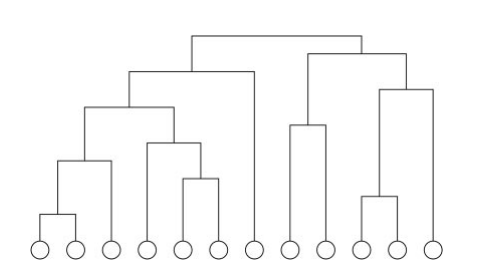
\includegraphics[width=\linewidth]{images/dendogram.png}
	\makebox[\textwidth][c]{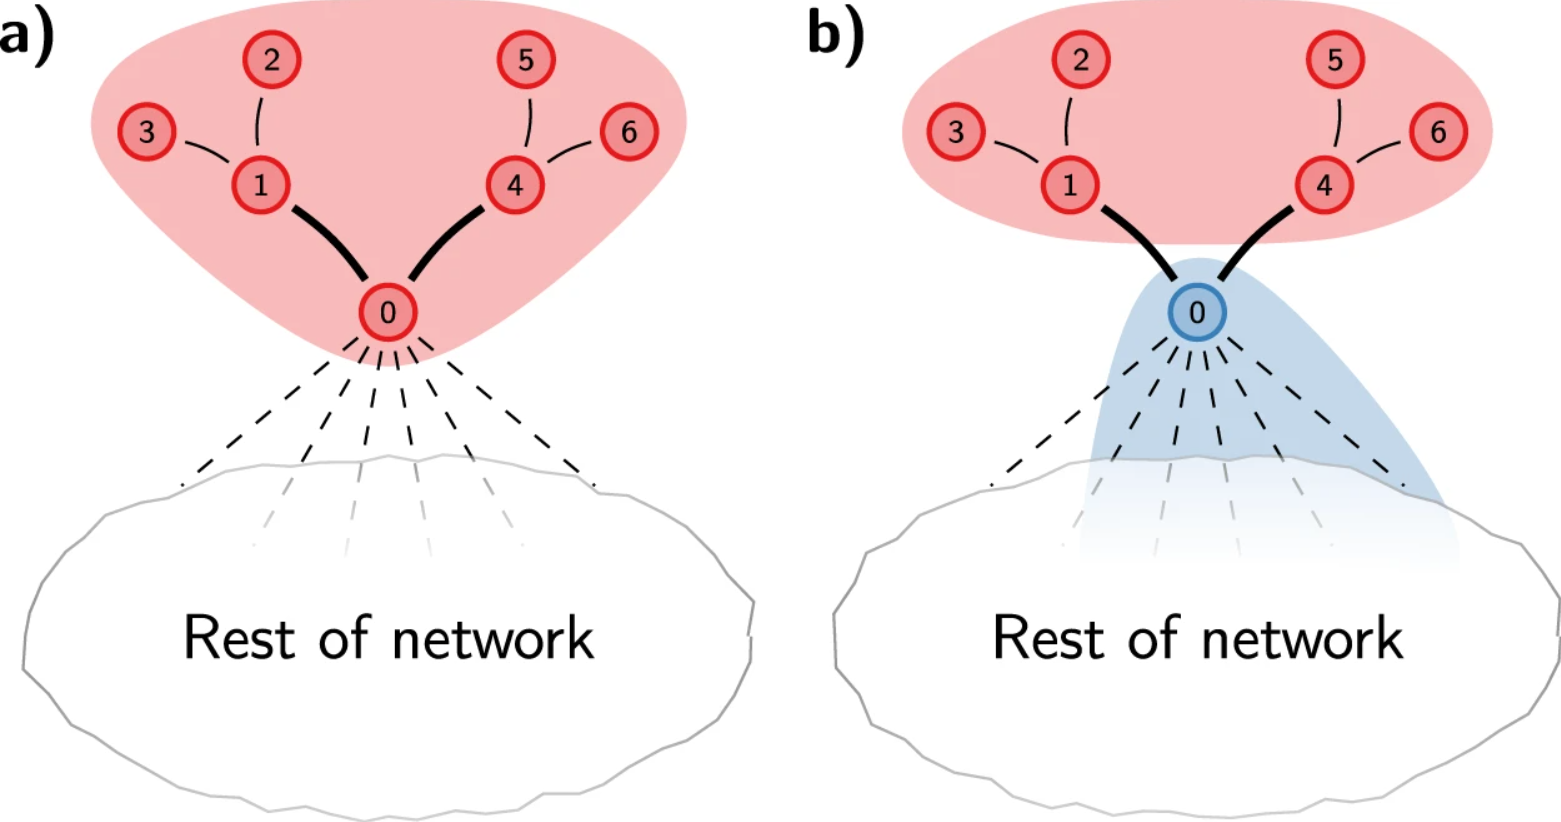
\includegraphics[width=0.8\textwidth]{images/bridge-node.png}}
	\caption{Primjer premještanja čvora iz zajednice u kojoj je predstavljao most između unutarnjih komponenti iz rada \cite{traag2019louvain}.}
	\label{fig:bridge-node}
\end{figure}


Leiden algoritam predstavljen je u radu \cite{traag2019louvain} 2019. godine te pokušava ispraviti nedostatke Louvaina korištenjem raznih, već poznatih strategija prilikom premještanja čvorova. Algoritam pametnog premještanja čvorova predstavljen je u radu \cite{waltman2013smart}. Leiden koristi ideju o ubrzavanju premještanja lokalnih iz rada \cite{ozaki2016simple} te ideju o premještanje čvora u zajednicu slučajno izabranog susjednog čvora iz rada \cite{traag2015faster}. Algoritam kao i Louvain radi premještanja na temelju optimizacije modularnosti.

Leiden algoritam sastoji se od tri faze: lokalno premještanje čvorova, pročišćavanje zajednica i agregacija mreže temeljena na pročišćenim zajednicama. U Louvain algoritmu agregacija zajednica u nove čvorove stvara se na temelju trenutnih zajednica. Leiden algoritam pokušava pročistiti pronađene zajednice prije koraka agregacije. Tim korakom zajednica se može podijeliti u podzajednice koje će bolje predstavljati strukturu mreže. Pročišćene zajednice se tada agregiraju u čvorove za iduću iteraciju algoritma. Podjela zajednica ostaje ista kakva je bila prije faze pročišćavanja, kao u Louvain algoritmu. Implementacijom faze pročišćavanja dobiva se bolja šansa da će algoritam pronaći zajednice visoke kvalitete i povezanosti.

Pročišćavanje se provodi na sličan način kao i prva faza algoritma, ali na razini zajednice. Svakom čvoru se dodijeli vlastita zajednica te se čvorovi lokalno spajaju sa drugima unutar zajednice ako su njihove veze dovoljno jake. Tijekom procesa pročišćavanja čvorovi se ne premještaju nužno pohlepno nego mogu biti dodani bilo kojoj zajednici za koju vrijednost funkcije kvalitete raste. Zajednica u koju će se čvor dodati odabire se slučajno, tako da je veća što je veći rast funkcije kvalitete. Razina slučajnosti ovisi o parametru $\theta > 0$. Slučajnost doprinosi istraživanju prostora zajednica i omogućava izlaženje iz potencijalnih lokalnih maksimuma. Isključivanje premještanja koja bi negativno utjecala na funkciju kvalitete nisu dozvoljena jer bi previše usporavala algoritam na velikim mrežama. Nakon faze pročišćavanja zajednica će vrlo često biti podijeljena, ali to ne mora nužno biti tako. 

Još jedna razlika u odnosu na Louvain algoritam događa se u procesu lokalnog premještanja čvorova. Leiden algoritam koristi implementaciju brzog premještanja. Algoritam posjećuje čvorove dok god postoje promjene u funkciji kvalitete. U ovakvom pristupu posjećuju se samo oni čvorovi kojima se dogodila promjena u susjedstvu za razliku od Louvaina koji u svakoj iteraciji obilazi sve čvorove. Proces započinje tako da se u red dodaju svi čvorovi mreže slučajnim poretkom. Tada se uzima prvi čvor te se provjerava raste li funkcija kvalitete premještanjem u neku zajednicu. Ako se čvor premjesti, na kraj reda dodaju se svi susjedi čvora koji ne pripadaju novoj zajednici, a nisu već u redu. Proces se nastavlja dokle god red nije prazan. Korištenjem brzog premještanja prva iteracija je ista kao u Louvain algoritmu i obilaze se svi čvorovi, ali se u kasnijim iteracijama posjećuju samo oni čvorovi na koje promjene zaista utječu čime Leiden algoritam postaje značajno efikasniji.


\begin{algorithm}
	\caption{Leiden algoritam}
	\begin{algorithmic}[1]
		\REQUIRE mreža G
		\REPEAT 
			\STATE{lokalno premještanje čvorova}
			 \IF{svaka zajednica se sastoji od samo jednog čvora} 
			 	\STATE {\textbf{break}} 
			 \ELSE
			 	\STATE pročistiti zajednice
			 	\STATE agregirati mrežu na temelji pročišćenih zajednica
			 	\STATE zadržati određeni raspored zajednica 
			 \ENDIF
		\UNTIL		
	\end{algorithmic}
\end{algorithm}


Razmisliti o primjeru na slici...


\section{Walktrap algoritam}



\chapter{Skupovi podataka}

U današnjem svijetu informacijski sustavi stvaraju goleme količine podataka. Podatke se može iskoristiti kako bi se poboljšali procesi koji se prate, pronašla područja u kojima postoji prostor za napredak, napraviti iskorak u poslovanju gdje se sustav primjenuje ili poboljšati korisničko iskustvo. Podaci su skupovi vrijednosti koji opisuju objekte u nekom procesu. Prate se kako bi se apstraktan proces iz ideje pretvorio u konkretne činjenice. Mogu se mjeriti, obrađivati i analizirati te vizualizirati kroz grafove, tablice i slike iz čega se dalje mogu izvoditi određeni zaključci. 


Algoritme koji se razvijaju da bi u podacima pronalazili korisne informacije potrebno je evaluirati te ocijeniti kako se ponašaju na kojem skupu podataka i pronaći situacije u kojima pokazuju najbolje performanse. Podaci prikupljeni iz stvarnih sustava najbolje opisuju praćene procese te je se najbolji zaključci mogu donijeti koristeći upravo njih.

Nakon problema i greški tijekom prikupljanja i praćenja osobnih podataka te loše sigurnosti i slučajeva krađe podataka, 2018. godine uvedena je uredba o općoj zaštiti podataka, poznata pod kraticom GDPR. Uredbom se kontrolira pohrana, prijenos i obrada osobnih podataka u Europskoj Uniji te su navedeni procesi znatno postroženi. Nakon Europske Unije slične odredbe primijenile su i neke američke savezne države te neke Azijske države čime odredba počinje vrijediti u gotovo svim razvijenijim dijelovima svijeta. Time je područje analiza društvenih mreža značajno pogođeno jer je postalo mnogo teže dobiti podatke o stvarnim korisnicima. Od tada značajnu ulogu počinju imati algoritmi za generiranje mreža koje imaju karakteristike društvenih zajednica. Algoritmi u početnom koraku dobivaju određene podatke o veličini i svojstvima željene mreže te generiraju takav primjer. U nastavku poglavlja opisat će se Watts-Strogatz model koji generira umjetne skupove podataka te stvarni skupovi podataka pomoću kojih će se algoritmi navedeni u radu testirati.



\section{Watts - Strogatz model}

Watts-Strogatz model predstavljen je u radu \cite{watts1998collective} 1998. godine. Autori su pokušali stvoriti algoritam koji će stvoriti umjetnu mrežu, koja će imati svojstva small-world mreža koje se mogu pronaći u primjenama u biološkim, tehnološkim i društvenim sustavima. Mreže takvih sustava nalaze se između dva ekstrema, slučajne mreže i pravilne rešetkaste mreže. Kako bi se generirala mreža koja je između ta dva slučaja može se iskoristiti proces slučajnog prespajanja bridova mreže. 

Proces započinje od pravilnog grafa prstenastog oblika sa $n$ vrhova i $k$ bridova po svakom vrhu te se svaki vrh prespaja s vjerojatnosti $p$. Vjerojatnost pruža mogućnost podešavanja oblika željenog grafa između regularnog za $p = 0$ i slučajnog za $p = 1$. Strukturna svojstva generiranog grafa mjere se pomoću karakteristične duljine puta, $L$ i koeficijenta grupiranja $C$. $L$ najčešće mjeri prosječnu duljinu puta u grafu i smatra se globalnim svojstvom grafa dok $C$ mjeri koliko su susjedne veze jake te se smatra lokalnim svojstvom. Za graf kada $p \rightarrow 1$ pokazuje se da normalizirane vrijednosti $L$ i $C$ teže prema 1 , dok kada $p \rightarrow 0$ $L$ i $C$ teže prema 0 što bi moglo značiti da je velika vrijednost $C$ povezana s velikim $L$, a mala vrijednost $C$ sa malom vrijednosti $L$. No graf na slici \ref{fig:C&L} pokazuje kako se vrijednosti $L$ i $C$ mijenjaju u ovisnosti o vjerojatnosti $p$ u odnosu na broj čvorova grafa. Vidljivo je kako postoji interval u kojem je $L$ malen gotovo kao $L_{random}$ dok je $C >> C_{random}$. Takva svojstva small-world mreže moguća su zbog neposrednog pada karakteristične duljine puta $L$ uvođenjem tek nekoliko slučajnih bridova. Efekt je visoko nelinearan te se za male vrijednosti $p$ brzo smanjuje udaljenost između vrhova, ali i zajednica. Za koeficijent grupiranja prespajanje ima tek linearan utjecaj te se koeficijent gotovo ne mijenja. 

\begin{figure}
	\makebox[\textwidth][c]{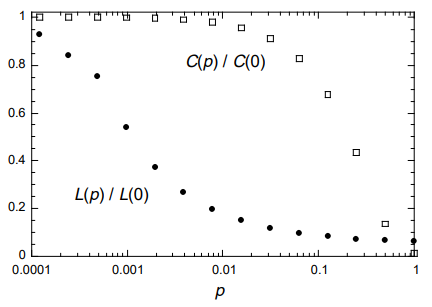
\includegraphics[width=0.7\textwidth]{images/C&L.png}}
	\caption{Karakteristična duljina puta $L$ i koeficijent grupiranja u grafovima s prespajanjem bridova u odnosu na normalizirane vrijednosti $L(0)$ i $C(0)$ za početni regularni graf.}
	\label{fig:C&L}
\end{figure}

U radu\cite{watts1998collective} ideja je provjerena na mnogo različitih početnih oblika mreža iz čega su nastali i podaci za graf \ref{fig:C&L}. Jedini uvjet je da bridovi koji se prespajaju moraju uglavnom povezivati vrhove za koje bi udaljenost bila mnogo veća nego u slučajnom grafu. Karakteristična duljina puta, $L(p)$ je definirana kao prosječna najkraća udaljenost između svih parova vrhova grafa. $C(p)$, koeficijent grupiranja, definiran je tako da ako čvor $v$ ima $k_{v}$ susjeda, onda među susjedima može postojati najviše $\frac{k_{v}(k_{v} - 1)}{2}$ bridova. Tada se $C_{v}$ definira kao omjer ostvarenih bridova među susjedima i ukupnog mogućeg broja bridova. Konačno $C$ se računa kao srednja vrijednost $C_{v}$ za svih $v$ vrhova grafa. U društvenim mrežama navedene mjere imaju smisleno značenje. $L$ je prosječan broj prijateljstava u lancu koji povezuje bilo koja dva člana zajednice. $C$ predstavlja koliko su prijatelji nekog člana zajednice povezani. Podaci prikazani u grafu \ref{fig:C&L} su uprosječeni rezultati 20 realizacija procesa slučajnog prespajanja vrhova grafa. Grafovi su imali po 1000 vrhova i prosječan stupanj vrha 10 po vrhu. Na horizontalnoj skali upotrijebljena je logaritamska skala kako bi se uspješno prikazao velik pad  $L$, dok $C$ ostaje konstantan kroz gotovo cijeli isječak koji graf prikazuje te ukazuje na činjenicu da je prelazak iz regularnog grafa prema small-world grafu gotovo neprimjetan na lokalnoj razini.


Algoritam generiranja modela grafa društvene zajednice sa small-world svojstvima odvija se kroz dva koraka. Algoritam prima tri parametra: $N$ predstavlja broj vrhova grafa, $k$ je srednja vrijednost stupnja pojedinog čvora i najčešće se odabire kao neki cijeli paran broj te $p$ što je parametar slučajnosti prespajanja promatranog brida grafa. Na konkretne parametre postoje određeni uvjeti. Vjerojatnost $p$ mora biti u granicama $0 \leq p \leq 1$. Parametri $N$ i $K$ moraju biti u sljedećem odnosu: $N >> K >> \log N >> 1$. Uvjetom $ K >> \log N$ garantira se da će generirani graf biti povezan \cite{Bollobas2001}. Algoritam konstruira neusmjereni graf sa $N$ čvorova i $\frac{NK}{2}$ bridova na sljedeći način:

\begin{enumerate}
	\item Konstruira se neusmjeren, regularan graf sa $N$ čvorova povezan sa $K$ susjeda, $\frac{K}{2}$ sa svake strane.
	\item Za svaki vrh promatra se svaki brid kojim je spojen s $\frac{K}{2}$ desnih susjeda i prespaja se s vjerojatnošću $p$. Prespajanje se obavlja tako da se brid spoji sa nekim od preostalih $v$ vrhova, različitih od trenutno promatranog i onoga s kojim ga je brid u tom trenutku povezivao, te između promatranog i odabranog vrha već ne postoji brid.
\end{enumerate}


\section{Stvarni podaci}

\chapter{Programsko ostvarenje}
...

\chapter{Vrednovanje i rezultati}
...

\chapter{Zaključak}

Detekcija zajednica u društvenim mrežama važan je i kompleksan zadatak koji primjenu pronalazi u različitim društvenim i tehničkim znanostima. Društvenih mreža postoji mnogo, od bioloških i informatičkih sustava do socijalnih društvenih mreža, ali nije jednostavno doći do stvarnih primjera podataka koji su zaštićeni strogim zakonima o korisničkoj privatnosti. Zato su umjetno generirane mreže postale važan dio u istraživanju ovog područja analize podataka. U radu je opisan Watts-Strogatz model koji generira mreže sa small-world svojstvima što odgovara svojstvima društvenih mreža u stvarnom svijetu.

Girvan-Newmanov algoritam prvi je algoritam osmišljen za pronalazak društvenih zajednica u kompleksnim mrežama. Osim što je daleko najpoznatiji algoritam detekcije zajednica, nakon njegovog predstavljanja pokrenuo se značajan rast i napredak u analizi društvenih mreža. Na temelju njega nastavljen je rad u ovom području te su razvijeni mnogi drugi algoritmi kojima je cilj bio poboljšati rezultate i ispraviti nedostatke Girvan-Newmanovog algoritma. Kroz rad se pokazalo da algoritam ipak ima određene nedostatke u vidu složenosti na zahtjevnijim društvenim mrežama te kako je za veće sustave potrebno potražiti bolja rješenja.

Kako bi se ustanovilo koji algoritmi daju najbolja rješenja, osim primjera društvenih mreža potrebne su i kvalitetne evaluacijske mjere. Njima se mjeri kvaliteta rješenja koje je algoritam pronašao. Najpoznatija mjera je modularnost čiju vrijednost optimiziraju čak tri od pet opisanih algoritama. U radu je opisano i korišteno devet mjera kojima se s Girvan-Newmanovim algoritmom usporedilo Louvain, Surprise, Leiden i Walktrap algoritme. Svi algoritmi su značajno niže složenosti te se Louvain algoritam pokazao najuspješnijim na svim evaluacijskim mjerama na umjetno generiranim podacima i stvarnim primjerima društvenih mreža. Leiden i Surprise algoritmi nastali su kao poboljšane verzije Louvaina. Surprise algoritam pokušava umjesto modularnosti iskoristiti mjeru surprise kako bi mjerio kvalitetu zajednica dok zadržava ostale korake Louvain algoritma. Leiden algoritam uvodi dodatne korake kojima se pokušava popraviti kvaliteta pronađenih zajednica. Algoritmi ipak nisu pokazali bolja svojstva te su potrebna dodatna usavršavanja kako bi dostigli razinu Louvain algoritma. Walktrap algortam koristi slučajne šetnje u grafu kojima pokušava pronaći zajednice, ali je nešto veće složenosti od svih algoritama, osim Girvan-Newmana te nije pokazao značajno bolje rezultate od ranije navednih algoritama. U programskoj implementaciji korištene su biblioteke NetworkX i SNAP koje pružaju implementacije algoritama te imaju dostupne primjere stvarnih društvenih mreža.

Budući radovi mogu uključivati izvođenje algoritama na snažnijoj računalnoj opremi, proučavanje novih algoritama te analizu algoritama uključivanjem dodatnih evaluacijskih mjera. Vrlo važni postaju umjetni izvori podataka koji bi generiranjem mreža sa svojstvima što sličnijim mrežama iz stvarnog života pružili dodatne mogućnosti u analizi. Također, postoji prostor za razvoj samih algoritama gdje bi se primjenom heurističkih metoda ili drugih metoda optimizacije korištenjem lokalnih svojstava grafova skratilo vrijeme izvođenja algoritma te omogućilo lakšu i bržu analizu i detekciju zajednica u zahtjevnim mrežama s milijunima korisnika.


\bibliographystyle{fer}
\bibliography{literatura.bib}


\begin{sazetak}
U radu je opisano pet algoritama za otkrivanje zajednica u društvenim mrežama. Pored najpoznatijeg Girvan-Newmanovog algoritma opisani su Louvain, Surprise, Leiden i Walktrap algoritmi. Kao dio rada implementirana je programska podrška koja pruža mogućnosti usporedbe algoritama i generiranja umjetnih mreža. Rezultati algoritama vrednovani su pomoću devet evaluacijskih mjera na umjetno generiranim mrežama, dobivenim pomoću Watts-Strogatz modela te na primjerima mreža iz stvarnog svijeta iz biblioteke SNAP. 

\kljucnerijeci{društvene mreže, otkrivanje zajednica, Girvan-Newman, Louvain, Surprise, Walktrap, small-world svojstva, Watts-Strogatz model}
\end{sazetak}

\engtitle{Comparing community detection algorithms in social networks}
\begin{abstract}
Thesis describes five community detection algorithms for finding communities in social networks. In addition to the most famous Girvan-Newman algorithm, there are described Louvain, Walktrap, Leiden and Walktrap algorithms. As part of the thesis there is implemented software which provides ability to compare algorithms and generate artificial networks. The results of algorithms are evaluated with nine evaluation measures on artificial networks that are created using Watts-Strogatz model and on the real world network examples from the SNAP library.

\keywords{social networks, community detection, Girvan-Newman, Louvain, Surprise, Leiden, Walktrap, small-world properties, Watts-Strogatz model}
\end{abstract}

\end{document}
